% CC-iGPT 整体架构图 (RGB-bit-exact, sub-pixel AR, R-only coarse)
% 编译: pdflatex ccigpt_arch.tex  (或 latexmk -pdf ccigpt_arch.tex)
% 也可独立嵌入论文: % CC-iGPT 整体架构图 (RGB-bit-exact, sub-pixel AR, R-only coarse)
% 编译: pdflatex ccigpt_arch.tex  (或 latexmk -pdf ccigpt_arch.tex)
% 也可独立嵌入论文: % CC-iGPT 整体架构图 (RGB-bit-exact, sub-pixel AR, R-only coarse)
% 编译: pdflatex ccigpt_arch.tex  (或 latexmk -pdf ccigpt_arch.tex)
% 也可独立嵌入论文: % CC-iGPT 整体架构图 (RGB-bit-exact, sub-pixel AR, R-only coarse)
% 编译: pdflatex ccigpt_arch.tex  (或 latexmk -pdf ccigpt_arch.tex)
% 也可独立嵌入论文: \input{figures/ccigpt_arch.tex}
\documentclass[tikz,border=8pt]{standalone}
\usepackage{tikz}
\usepackage{amsmath,amssymb}
\usetikzlibrary{positioning,arrows.meta,calc,fit,backgrounds,shapes.geometric,decorations.pathreplacing}

\begin{document}
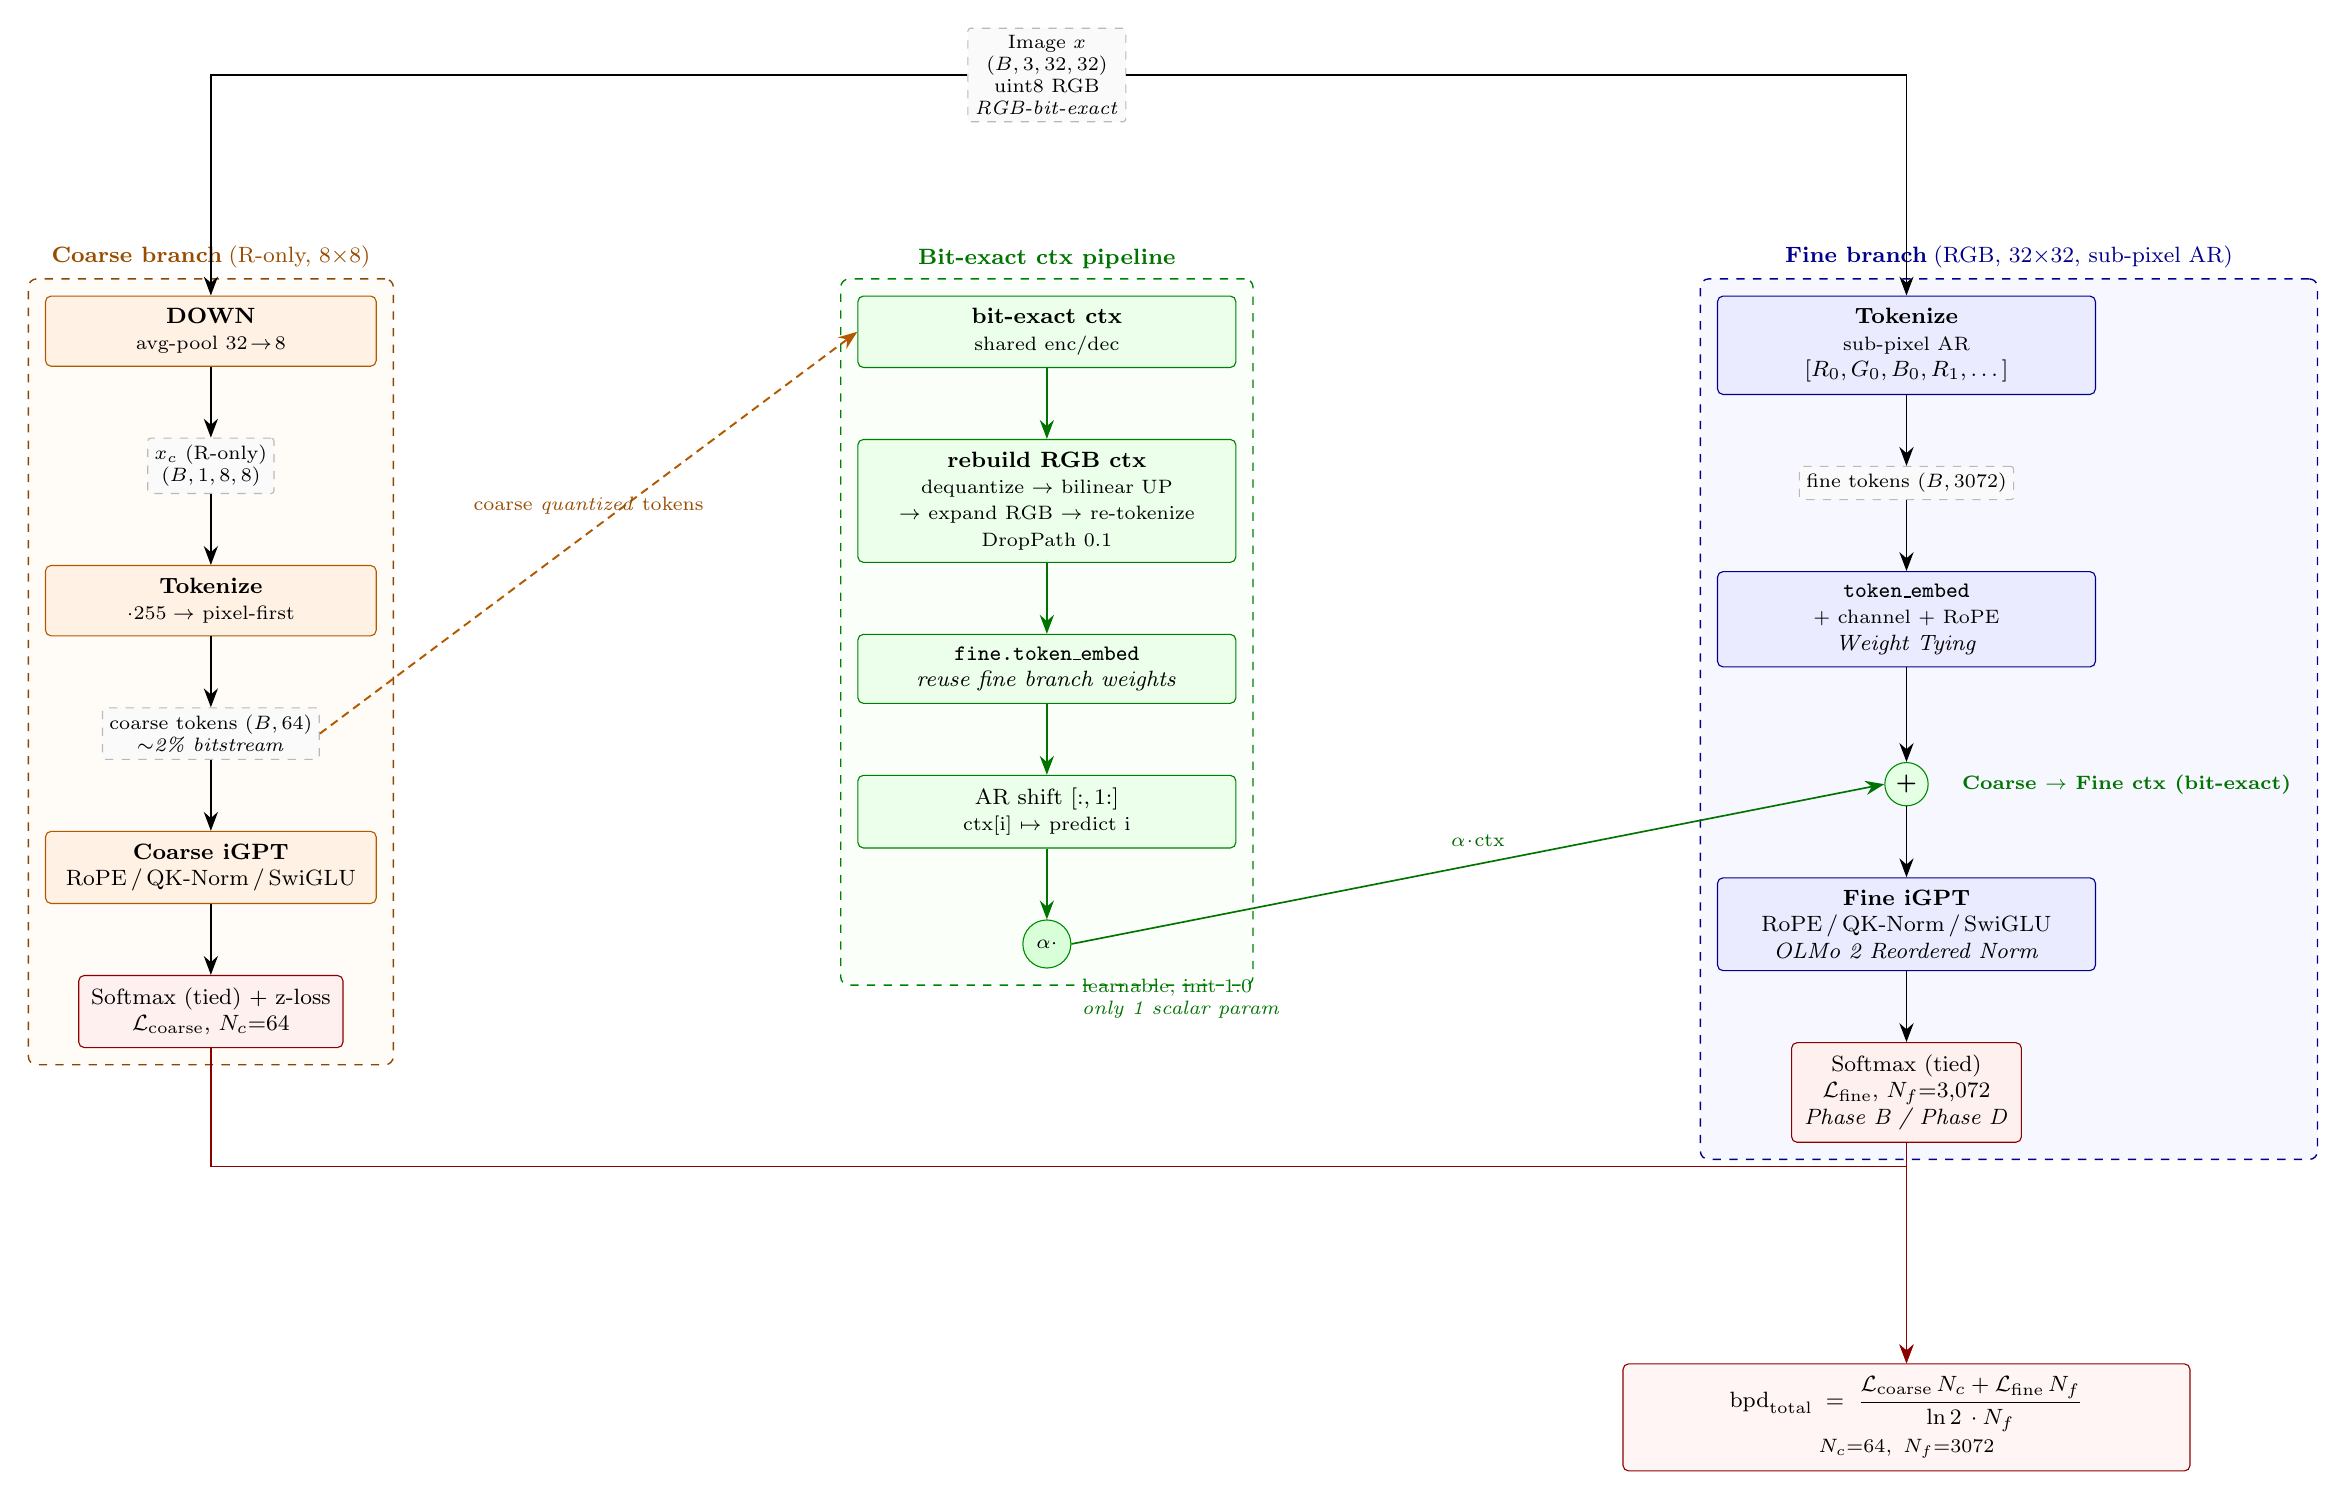
\begin{tikzpicture}[
    font=\footnotesize,
    >={Stealth[length=2.4mm]},
    node distance=9mm and 18mm, % 进一步优化间距
    % 模块样式
    blk/.style    ={draw, rounded corners=2pt, align=center,
                    minimum height=8mm, inner sep=4.5pt,
                    fill=blue!6, draw=blue!55!black, line width=0.4pt},
    coarseblk/.style={blk, fill=orange!10, draw=orange!70!black, minimum width=42mm},
    fineblk/.style  ={blk, fill=blue!8,   draw=blue!55!black,   minimum width=48mm},
    ctxblk/.style   ={blk, fill=green!8,  draw=green!50!black, minimum width=48mm},
    lossblk/.style  ={draw, rounded corners=2pt, align=center, fill=red!6,
                      draw=red!55!black, minimum height=8mm, inner sep=4.5pt},
    tensor/.style ={draw, dashed, rounded corners=1pt, align=center,
                    fill=gray!4, draw=gray!55, font=\scriptsize, inner sep=2.5pt},
    pillar/.style ={draw, rounded corners=3pt, dashed, line width=0.5pt,
                    inner sep=6pt}, % 增加pillar内边距
    flow/.style   ={->, line width=0.5pt},
    ctxflow/.style={->, line width=0.6pt, green!45!black},
    biteq/.style  ={->, line width=0.7pt, orange!70!black, densely dashed},
]

% ============================================================
% INPUT (顶部居中)
% ============================================================
\node[tensor] (x) {Image $x$\\$(B,3,32,32)$\\ uint8 RGB\\\textit{RGB-bit-exact}};

% ============================================================
% LEFT COLUMN — COARSE BRANCH (R-only 8x8)
% ============================================================
\node[coarseblk, below left=22mm and 75mm of x] (down)
    {\textbf{DOWN}\\\scriptsize avg-pool $32\!\to\!8$};

\node[tensor, below=of down] (xc)
    {$x_c$ (R-only)\\$(B,1,8,8)$};

\node[coarseblk, below=of xc] (ctok)
    {\textbf{Tokenize}\\\scriptsize$\cdot255 \to $ pixel-first};

\node[tensor, below=of ctok] (ctokens)
    {coarse tokens $(B,64)$\\\textit{$\sim$2\% bitstream}};

\node[coarseblk, below=of ctokens] (coarse)
    {\textbf{Coarse iGPT}\\
     RoPE\,/\,QK-Norm\,/\,SwiGLU};

\node[lossblk, below=of coarse] (cehead_c)
    {Softmax (tied) $+$ z-loss\\
     $\mathcal{L}_{\text{coarse}}$, $N_c{=}64$};

% ============================================================
% MIDDLE COLUMN — CTX PIPELINE (bit-exact) 【正中间】
% ============================================================
\node[ctxblk, below=22mm of x, xshift=0mm, align=center] (ctxstart)
    {\textbf{bit-exact ctx}\\\scriptsize shared enc/dec};
\node[ctxblk, below=of ctxstart] (rebuild)
    {\textbf{rebuild RGB ctx}\\
     \scriptsize dequantize $\to$ bilinear UP\\
     \scriptsize $\to$ expand RGB $\to$ re-tokenize\\
     \scriptsize DropPath 0.1};
\node[ctxblk, below=of rebuild] (embed)
    {\texttt{fine.token\_embed}\\\textit{reuse fine branch weights}};
\node[ctxblk, below=of embed] (shift)
    {AR shift $[:,1{:}]$\\\scriptsize ctx[i] $\mapsto$ predict i};

\node[draw, circle, fill=green!15, draw=green!55!black, minimum size=6mm,
      below=of shift] (alpha) {\scriptsize$\alpha\cdot$};
% 调整文字位置到alpha右下方
\node[font=\scriptsize, below right=1mm and 1mm of alpha, text=green!45!black, align=left]
     {learnable, init 1.0\\\textit{only 1 scalar param}};

% ============================================================
% RIGHT COLUMN — FINE BRANCH (32x32 sub-pixel AR)
% ============================================================
\node[fineblk, below right=22mm and 75mm of x] (ftok)
    {\textbf{Tokenize}\\\scriptsize sub-pixel AR\\$[R_0,G_0,B_0,R_1,\dots]$};

\node[tensor, below=of ftok] (ftokens)
    {fine tokens $(B,3072)$};

\node[fineblk, below=of ftokens] (tokemb)
    {\texttt{token\_embed}\\\scriptsize $+$ channel $+$ RoPE\\\textit{Weight Tying}};

% --- α 注入交汇点 ---
\node[draw, circle, inner sep=0.6pt, fill=green!10, draw=green!55!black,
      minimum size=5.5mm, below=12mm of tokemb] (plus) {$\boldsymbol{+}$};

% 关键修改：将标签放在绿色加号圆形的右边
\node[font=\scriptsize, right=3mm of plus, text=green!45!black, anchor=west]
     (ctxlabel) {\textbf{Coarse $\to$ Fine ctx (bit-exact)}};

\node[fineblk, below=of plus] (fine)
    {\textbf{Fine iGPT}\\
     RoPE\,/\,QK-Norm\,/\,SwiGLU\\\textit{OLMo 2 Reordered Norm}};

\node[lossblk, below=of fine] (cehead_f)
    {Softmax (tied)\\
     $\mathcal{L}_{\text{fine}}$, $N_f{=}3{,}072$\\\textit{Phase B / Phase D}};

% ============================================================
% BPD AGGREGATION (底部居中)
% ============================================================
\node[lossblk, fill=red!4, below=28mm of cehead_f, minimum width=72mm] (bpd)
    {$\displaystyle
        \mathrm{bpd}_{\text{total}}
        \;=\;\frac{\mathcal{L}_{\text{coarse}}\,N_c + \mathcal{L}_{\text{fine}}\,N_f}{\ln 2\,\cdot N_f}$
    \\[2pt]\scriptsize $N_c{=}64,\ N_f{=}3072$};

% ============================================================
% EDGES — main flow (彻底优化路径，无任何重叠)
% ============================================================
% input split
\draw[flow] (x) -| (down);
\draw[flow] (x) -| (ftok);

% coarse column
\draw[flow] (down)    -- (xc);
\draw[flow] (xc)      -- (ctok);
\draw[flow] (ctok)    -- (ctokens);
\draw[flow] (ctokens) -- (coarse);
\draw[flow] (coarse)  -- (cehead_c);

% fine column
\draw[flow] (ftok)    -- (ftokens);
\draw[flow] (ftokens) -- (tokemb);
\draw[flow] (tokemb)  -- (plus);
\draw[flow] (plus)    -- (fine);
\draw[flow] (fine)    -- (cehead_f);

% ctx bit-exact pipeline (关键修复：直接水平连接，无直角弯)
\draw[biteq] (ctokens.east) -- node[above,font=\scriptsize,orange!60!black, yshift=1mm]
            {coarse \emph{quantized} tokens}(ctxstart.west);
\draw[ctxflow] (ctxstart) -- (rebuild);
\draw[ctxflow] (rebuild)  -- (embed);
\draw[ctxflow] (embed)    -- (shift);
\draw[ctxflow] (shift)    -- (alpha);
% 只保留α·ctx标签在箭头上方
\draw[ctxflow] (alpha.east) -- node[above,font=\scriptsize,green!40!black, yshift=1mm]
              {$\alpha\!\cdot\!\mathrm{ctx}$} (plus.west);

% loss aggregation (关键修复：箭头直接指向block，无多余拐弯)
\draw[flow, red!55!black] (cehead_c.south) -- ++(0,-15mm) -| (bpd.north);
\draw[flow, red!55!black] (cehead_f.south) -- ++(0,-15mm) -| (bpd.north);

% ============================================================
% PILLAR BOXES (visual grouping)
% ============================================================
\begin{pgfonlayer}{background}
  \node[pillar, draw=orange!55!black, fill=orange!3,
        fit=(down)(xc)(ctok)(ctokens)(coarse)(cehead_c),
        label={[orange!60!black]above:\textbf{Coarse branch}\;(R-only, 8$\times$8)}]
        (coarsebox) {};
  \node[pillar, draw=green!50!black, fill=green!2, dashed,
        fit=(ctxstart)(rebuild)(embed)(shift)(alpha),
        label={[green!45!black]above:\textbf{Bit-exact ctx pipeline}}]
        (ctxbox) {};
  \node[pillar, draw=blue!55!black, fill=blue!3,
        fit=(ftok)(ftokens)(tokemb)(plus)(ctxlabel)(fine)(cehead_f),
        label={[blue!55!black]above:\textbf{Fine branch}\;(RGB, 32$\times$32, sub-pixel AR)}]
        (finebox) {};
\end{pgfonlayer}

\end{tikzpicture}
\end{document}
\documentclass[tikz,border=8pt]{standalone}
\usepackage{tikz}
\usepackage{amsmath,amssymb}
\usetikzlibrary{positioning,arrows.meta,calc,fit,backgrounds,shapes.geometric,decorations.pathreplacing}

\begin{document}
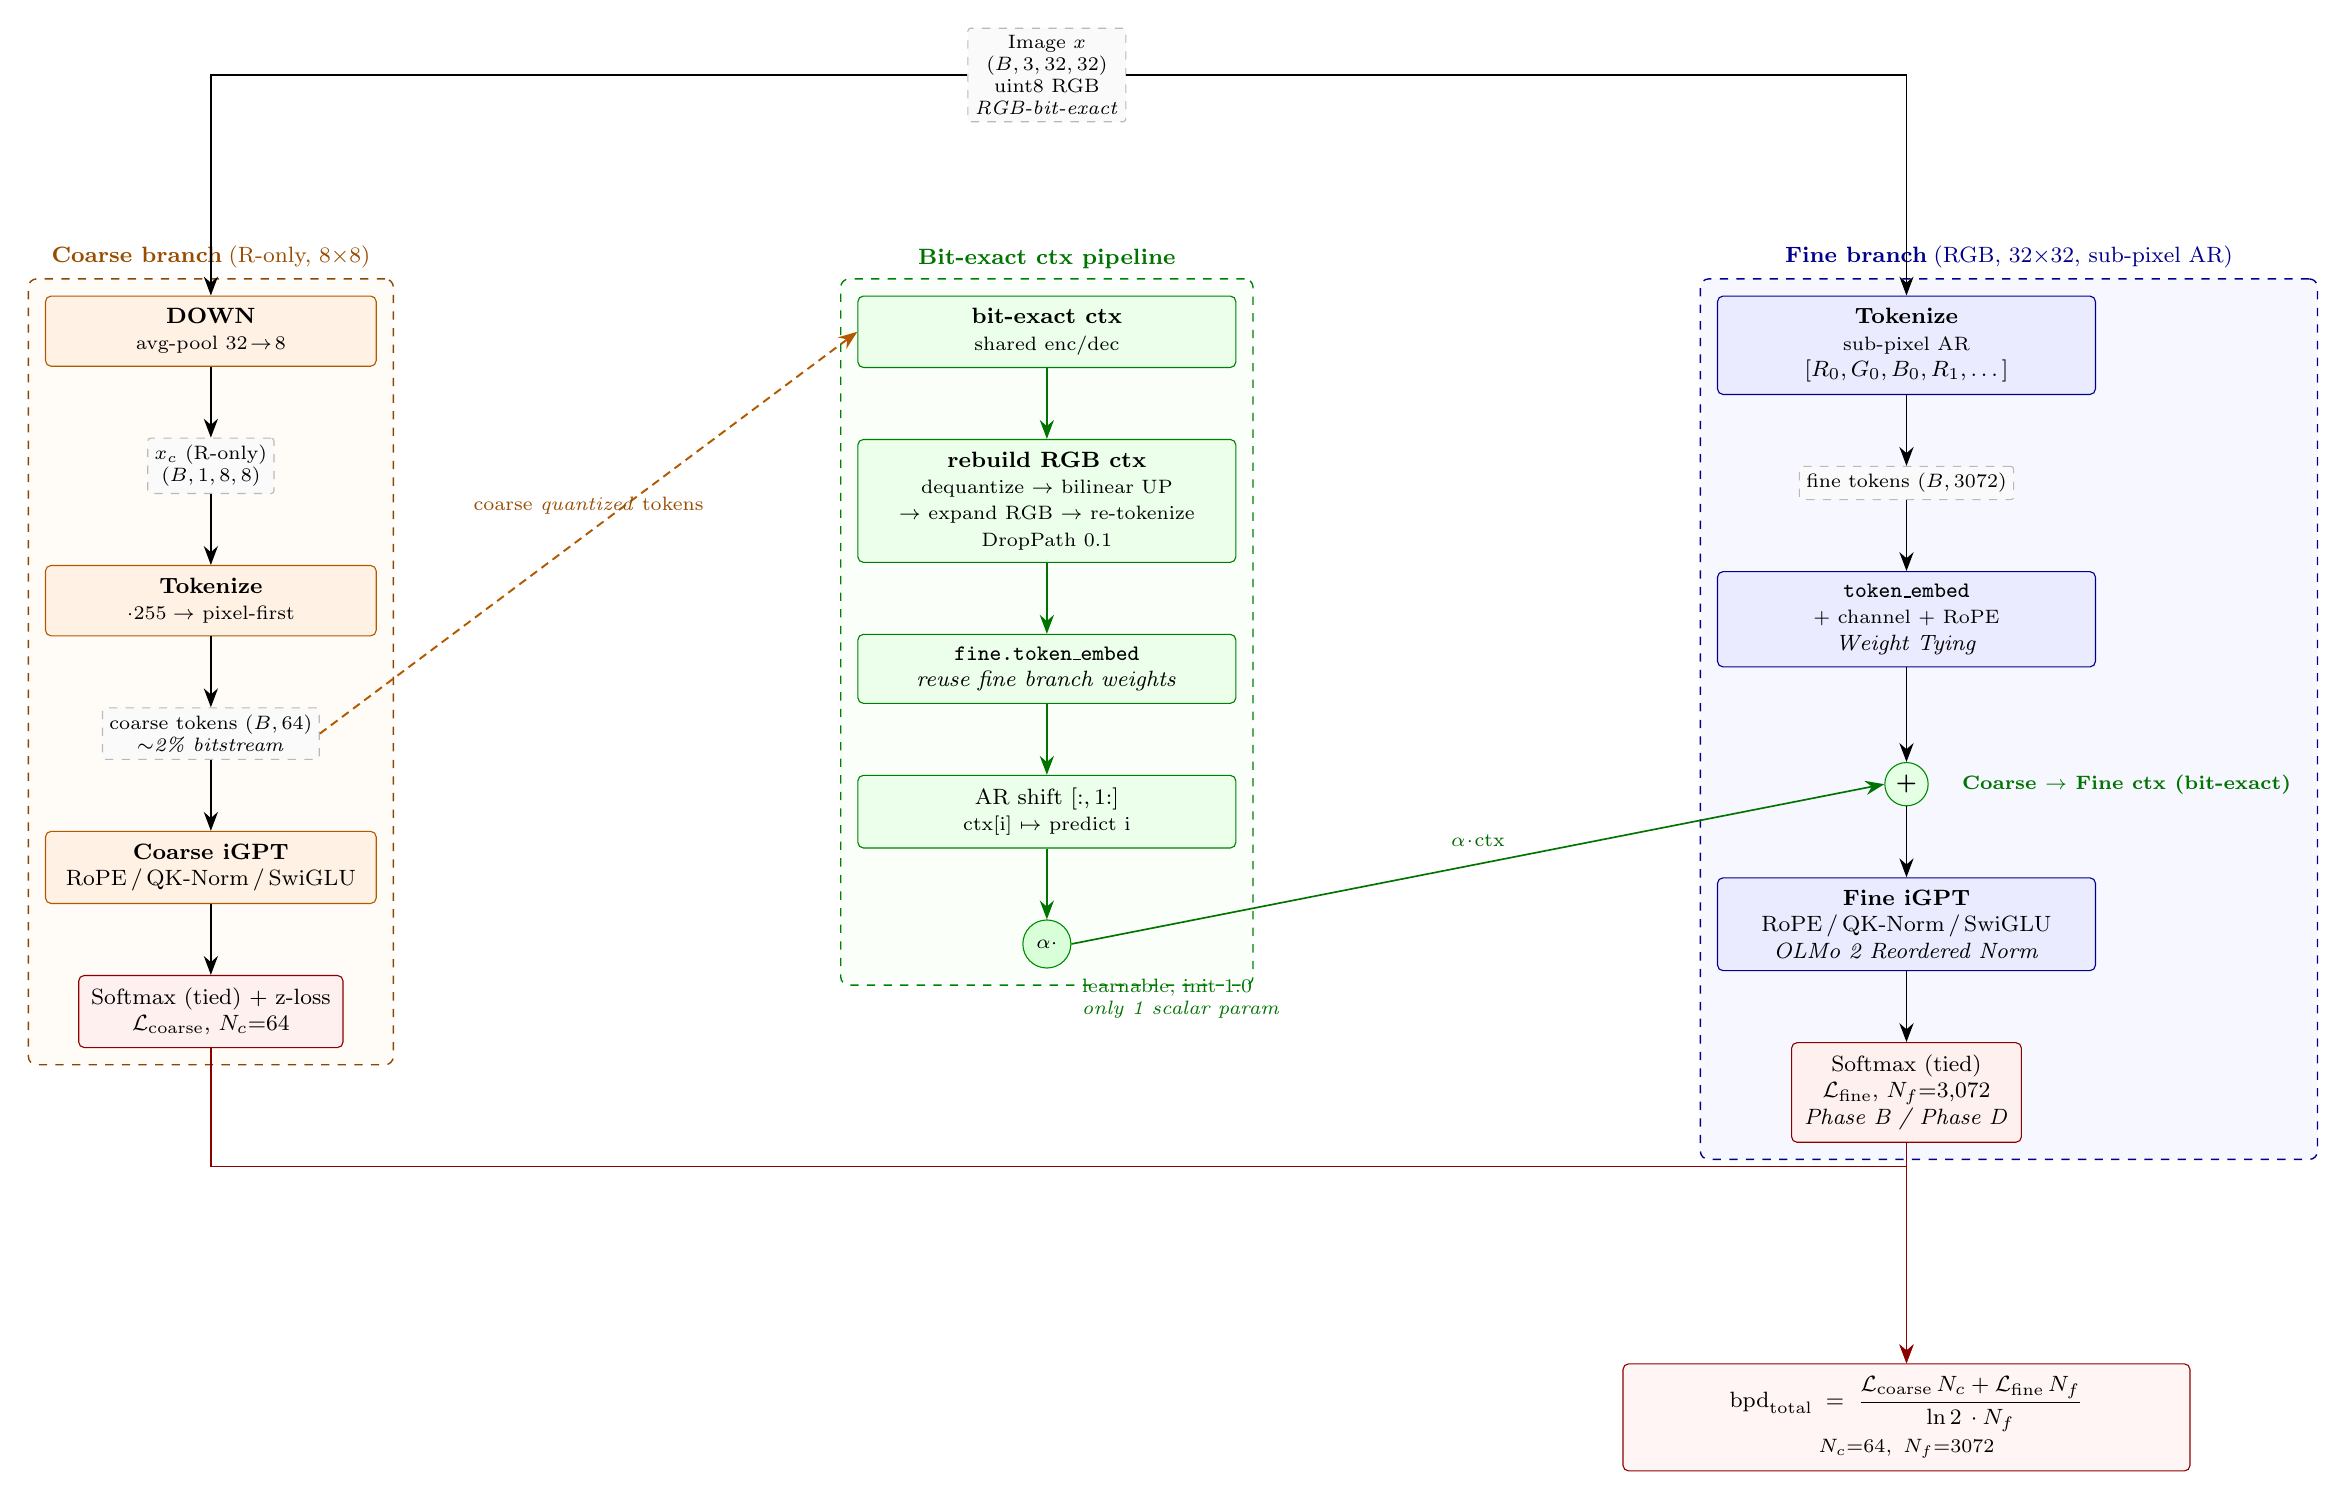
\begin{tikzpicture}[
    font=\footnotesize,
    >={Stealth[length=2.4mm]},
    node distance=9mm and 18mm, % 进一步优化间距
    % 模块样式
    blk/.style    ={draw, rounded corners=2pt, align=center,
                    minimum height=8mm, inner sep=4.5pt,
                    fill=blue!6, draw=blue!55!black, line width=0.4pt},
    coarseblk/.style={blk, fill=orange!10, draw=orange!70!black, minimum width=42mm},
    fineblk/.style  ={blk, fill=blue!8,   draw=blue!55!black,   minimum width=48mm},
    ctxblk/.style   ={blk, fill=green!8,  draw=green!50!black, minimum width=48mm},
    lossblk/.style  ={draw, rounded corners=2pt, align=center, fill=red!6,
                      draw=red!55!black, minimum height=8mm, inner sep=4.5pt},
    tensor/.style ={draw, dashed, rounded corners=1pt, align=center,
                    fill=gray!4, draw=gray!55, font=\scriptsize, inner sep=2.5pt},
    pillar/.style ={draw, rounded corners=3pt, dashed, line width=0.5pt,
                    inner sep=6pt}, % 增加pillar内边距
    flow/.style   ={->, line width=0.5pt},
    ctxflow/.style={->, line width=0.6pt, green!45!black},
    biteq/.style  ={->, line width=0.7pt, orange!70!black, densely dashed},
]

% ============================================================
% INPUT (顶部居中)
% ============================================================
\node[tensor] (x) {Image $x$\\$(B,3,32,32)$\\ uint8 RGB\\\textit{RGB-bit-exact}};

% ============================================================
% LEFT COLUMN — COARSE BRANCH (R-only 8x8)
% ============================================================
\node[coarseblk, below left=22mm and 75mm of x] (down)
    {\textbf{DOWN}\\\scriptsize avg-pool $32\!\to\!8$};

\node[tensor, below=of down] (xc)
    {$x_c$ (R-only)\\$(B,1,8,8)$};

\node[coarseblk, below=of xc] (ctok)
    {\textbf{Tokenize}\\\scriptsize$\cdot255 \to $ pixel-first};

\node[tensor, below=of ctok] (ctokens)
    {coarse tokens $(B,64)$\\\textit{$\sim$2\% bitstream}};

\node[coarseblk, below=of ctokens] (coarse)
    {\textbf{Coarse iGPT}\\
     RoPE\,/\,QK-Norm\,/\,SwiGLU};

\node[lossblk, below=of coarse] (cehead_c)
    {Softmax (tied) $+$ z-loss\\
     $\mathcal{L}_{\text{coarse}}$, $N_c{=}64$};

% ============================================================
% MIDDLE COLUMN — CTX PIPELINE (bit-exact) 【正中间】
% ============================================================
\node[ctxblk, below=22mm of x, xshift=0mm, align=center] (ctxstart)
    {\textbf{bit-exact ctx}\\\scriptsize shared enc/dec};
\node[ctxblk, below=of ctxstart] (rebuild)
    {\textbf{rebuild RGB ctx}\\
     \scriptsize dequantize $\to$ bilinear UP\\
     \scriptsize $\to$ expand RGB $\to$ re-tokenize\\
     \scriptsize DropPath 0.1};
\node[ctxblk, below=of rebuild] (embed)
    {\texttt{fine.token\_embed}\\\textit{reuse fine branch weights}};
\node[ctxblk, below=of embed] (shift)
    {AR shift $[:,1{:}]$\\\scriptsize ctx[i] $\mapsto$ predict i};

\node[draw, circle, fill=green!15, draw=green!55!black, minimum size=6mm,
      below=of shift] (alpha) {\scriptsize$\alpha\cdot$};
% 调整文字位置到alpha右下方
\node[font=\scriptsize, below right=1mm and 1mm of alpha, text=green!45!black, align=left]
     {learnable, init 1.0\\\textit{only 1 scalar param}};

% ============================================================
% RIGHT COLUMN — FINE BRANCH (32x32 sub-pixel AR)
% ============================================================
\node[fineblk, below right=22mm and 75mm of x] (ftok)
    {\textbf{Tokenize}\\\scriptsize sub-pixel AR\\$[R_0,G_0,B_0,R_1,\dots]$};

\node[tensor, below=of ftok] (ftokens)
    {fine tokens $(B,3072)$};

\node[fineblk, below=of ftokens] (tokemb)
    {\texttt{token\_embed}\\\scriptsize $+$ channel $+$ RoPE\\\textit{Weight Tying}};

% --- α 注入交汇点 ---
\node[draw, circle, inner sep=0.6pt, fill=green!10, draw=green!55!black,
      minimum size=5.5mm, below=12mm of tokemb] (plus) {$\boldsymbol{+}$};

% 关键修改：将标签放在绿色加号圆形的右边
\node[font=\scriptsize, right=3mm of plus, text=green!45!black, anchor=west]
     (ctxlabel) {\textbf{Coarse $\to$ Fine ctx (bit-exact)}};

\node[fineblk, below=of plus] (fine)
    {\textbf{Fine iGPT}\\
     RoPE\,/\,QK-Norm\,/\,SwiGLU\\\textit{OLMo 2 Reordered Norm}};

\node[lossblk, below=of fine] (cehead_f)
    {Softmax (tied)\\
     $\mathcal{L}_{\text{fine}}$, $N_f{=}3{,}072$\\\textit{Phase B / Phase D}};

% ============================================================
% BPD AGGREGATION (底部居中)
% ============================================================
\node[lossblk, fill=red!4, below=28mm of cehead_f, minimum width=72mm] (bpd)
    {$\displaystyle
        \mathrm{bpd}_{\text{total}}
        \;=\;\frac{\mathcal{L}_{\text{coarse}}\,N_c + \mathcal{L}_{\text{fine}}\,N_f}{\ln 2\,\cdot N_f}$
    \\[2pt]\scriptsize $N_c{=}64,\ N_f{=}3072$};

% ============================================================
% EDGES — main flow (彻底优化路径，无任何重叠)
% ============================================================
% input split
\draw[flow] (x) -| (down);
\draw[flow] (x) -| (ftok);

% coarse column
\draw[flow] (down)    -- (xc);
\draw[flow] (xc)      -- (ctok);
\draw[flow] (ctok)    -- (ctokens);
\draw[flow] (ctokens) -- (coarse);
\draw[flow] (coarse)  -- (cehead_c);

% fine column
\draw[flow] (ftok)    -- (ftokens);
\draw[flow] (ftokens) -- (tokemb);
\draw[flow] (tokemb)  -- (plus);
\draw[flow] (plus)    -- (fine);
\draw[flow] (fine)    -- (cehead_f);

% ctx bit-exact pipeline (关键修复：直接水平连接，无直角弯)
\draw[biteq] (ctokens.east) -- node[above,font=\scriptsize,orange!60!black, yshift=1mm]
            {coarse \emph{quantized} tokens}(ctxstart.west);
\draw[ctxflow] (ctxstart) -- (rebuild);
\draw[ctxflow] (rebuild)  -- (embed);
\draw[ctxflow] (embed)    -- (shift);
\draw[ctxflow] (shift)    -- (alpha);
% 只保留α·ctx标签在箭头上方
\draw[ctxflow] (alpha.east) -- node[above,font=\scriptsize,green!40!black, yshift=1mm]
              {$\alpha\!\cdot\!\mathrm{ctx}$} (plus.west);

% loss aggregation (关键修复：箭头直接指向block，无多余拐弯)
\draw[flow, red!55!black] (cehead_c.south) -- ++(0,-15mm) -| (bpd.north);
\draw[flow, red!55!black] (cehead_f.south) -- ++(0,-15mm) -| (bpd.north);

% ============================================================
% PILLAR BOXES (visual grouping)
% ============================================================
\begin{pgfonlayer}{background}
  \node[pillar, draw=orange!55!black, fill=orange!3,
        fit=(down)(xc)(ctok)(ctokens)(coarse)(cehead_c),
        label={[orange!60!black]above:\textbf{Coarse branch}\;(R-only, 8$\times$8)}]
        (coarsebox) {};
  \node[pillar, draw=green!50!black, fill=green!2, dashed,
        fit=(ctxstart)(rebuild)(embed)(shift)(alpha),
        label={[green!45!black]above:\textbf{Bit-exact ctx pipeline}}]
        (ctxbox) {};
  \node[pillar, draw=blue!55!black, fill=blue!3,
        fit=(ftok)(ftokens)(tokemb)(plus)(ctxlabel)(fine)(cehead_f),
        label={[blue!55!black]above:\textbf{Fine branch}\;(RGB, 32$\times$32, sub-pixel AR)}]
        (finebox) {};
\end{pgfonlayer}

\end{tikzpicture}
\end{document}
\documentclass[tikz,border=8pt]{standalone}
\usepackage{tikz}
\usepackage{amsmath,amssymb}
\usetikzlibrary{positioning,arrows.meta,calc,fit,backgrounds,shapes.geometric,decorations.pathreplacing}

\begin{document}
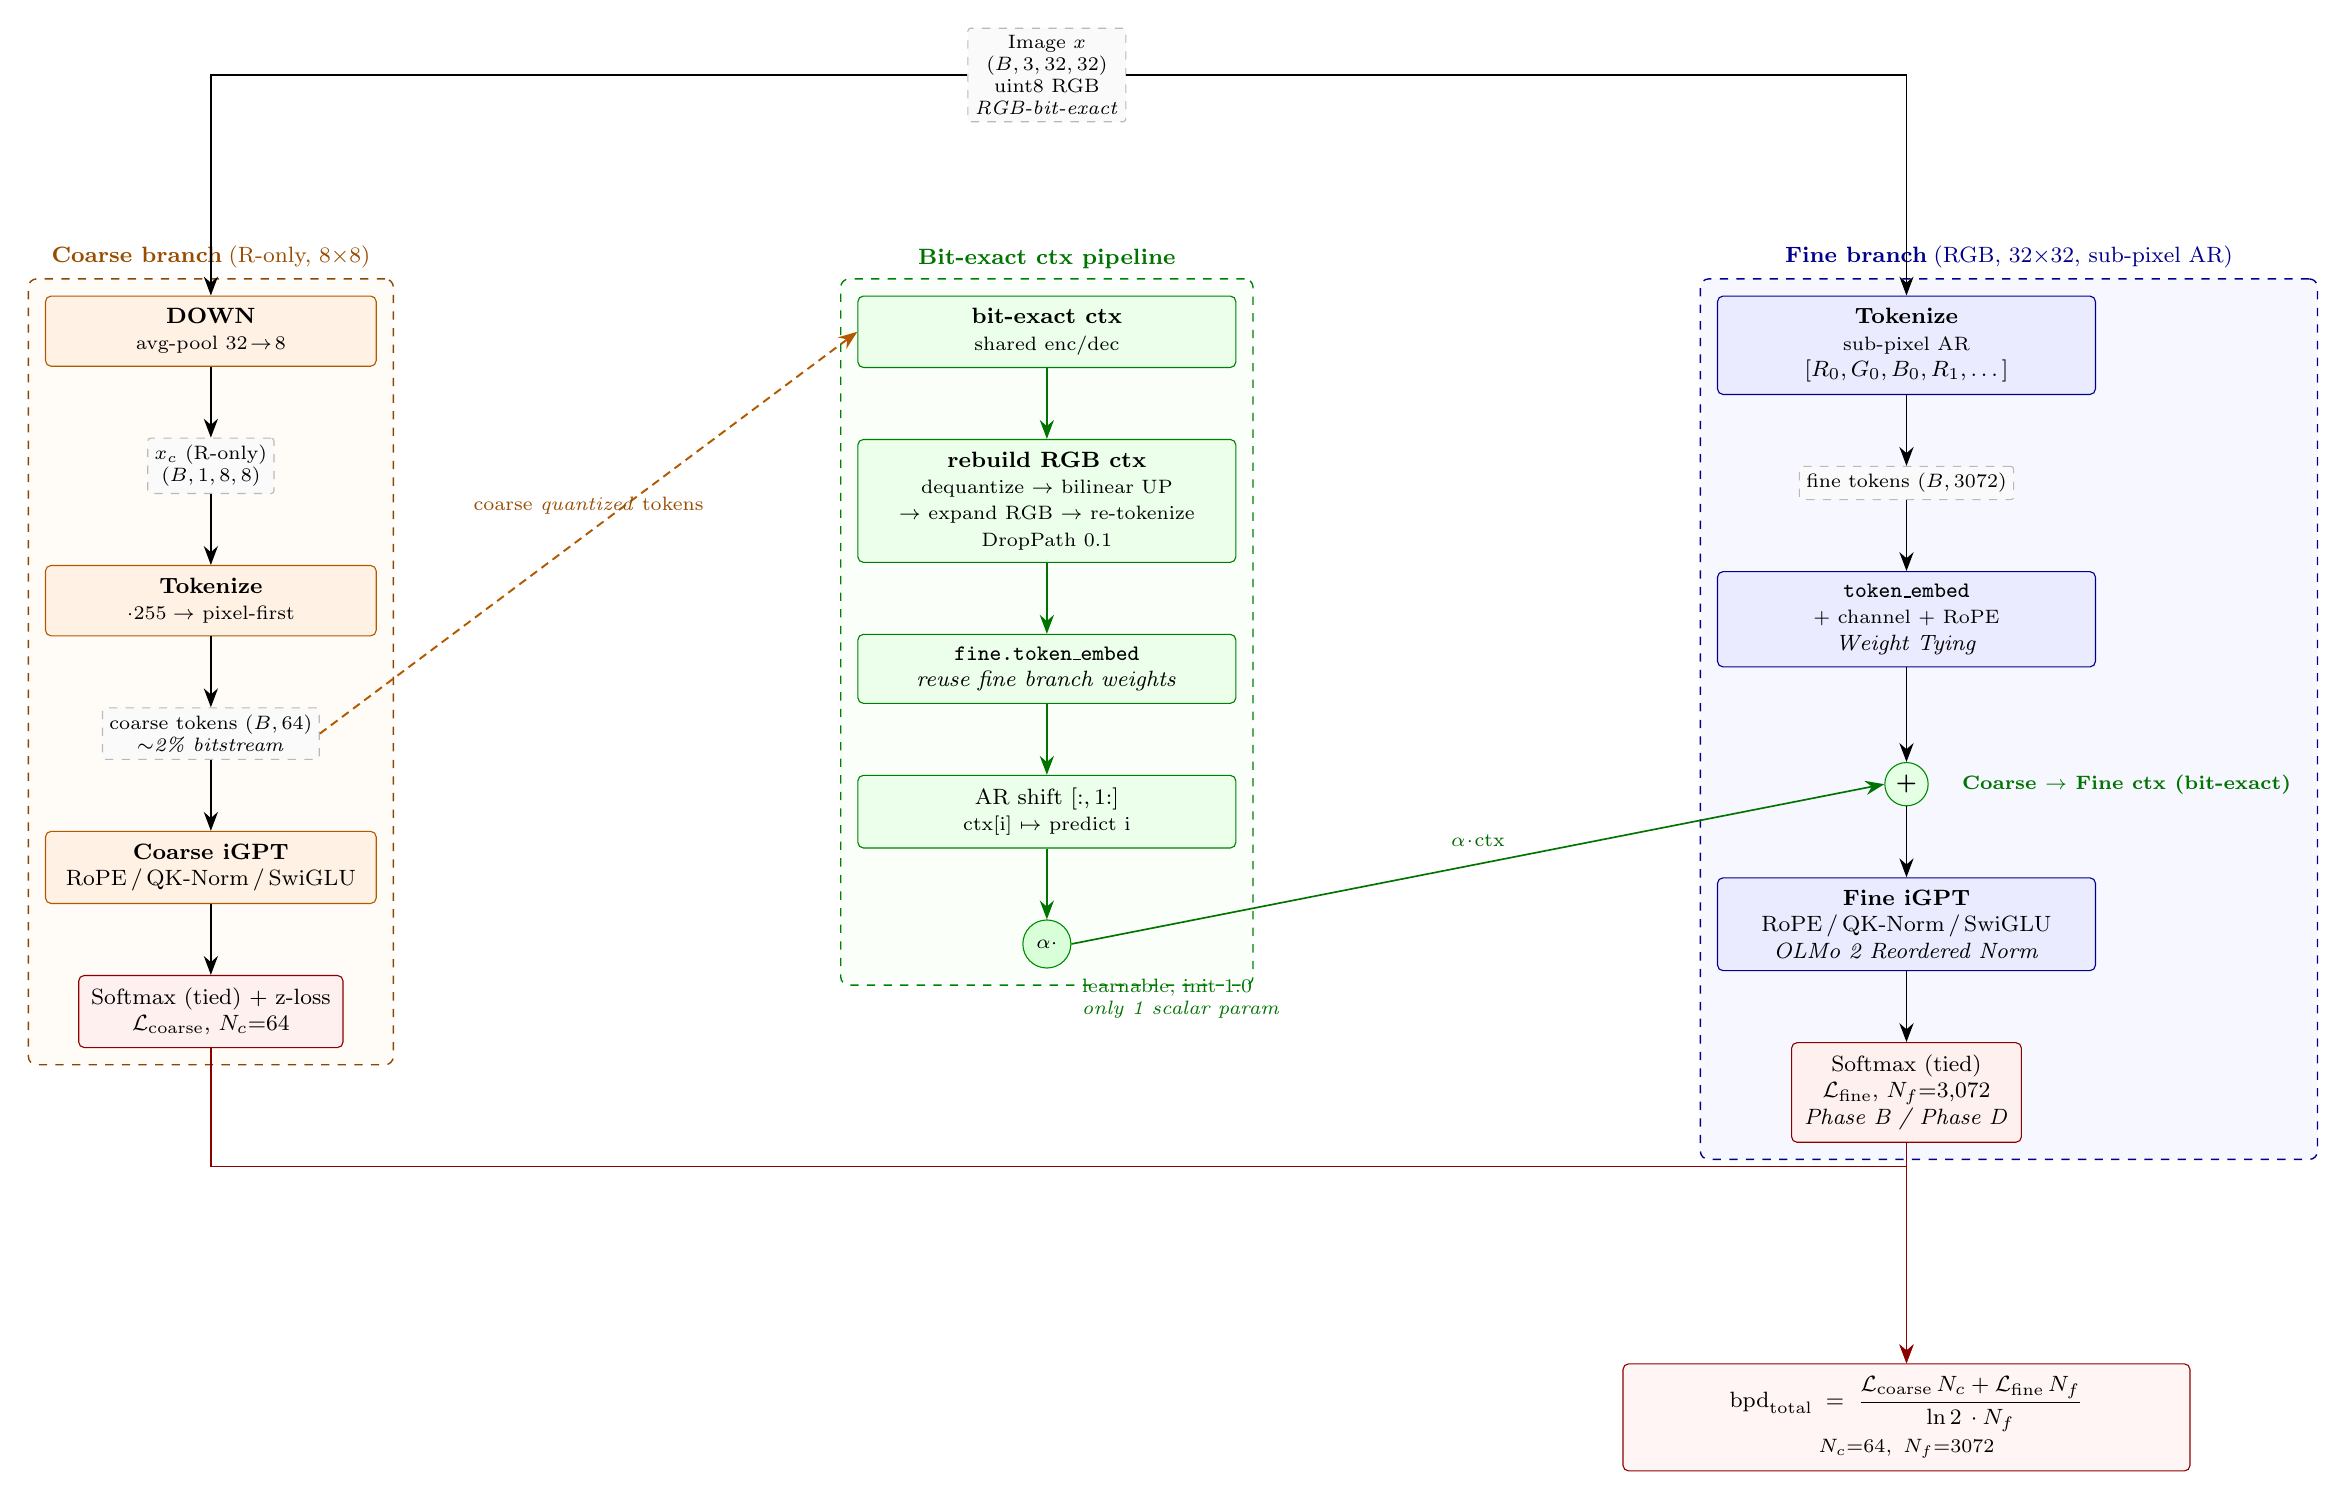
\begin{tikzpicture}[
    font=\footnotesize,
    >={Stealth[length=2.4mm]},
    node distance=9mm and 18mm, % 进一步优化间距
    % 模块样式
    blk/.style    ={draw, rounded corners=2pt, align=center,
                    minimum height=8mm, inner sep=4.5pt,
                    fill=blue!6, draw=blue!55!black, line width=0.4pt},
    coarseblk/.style={blk, fill=orange!10, draw=orange!70!black, minimum width=42mm},
    fineblk/.style  ={blk, fill=blue!8,   draw=blue!55!black,   minimum width=48mm},
    ctxblk/.style   ={blk, fill=green!8,  draw=green!50!black, minimum width=48mm},
    lossblk/.style  ={draw, rounded corners=2pt, align=center, fill=red!6,
                      draw=red!55!black, minimum height=8mm, inner sep=4.5pt},
    tensor/.style ={draw, dashed, rounded corners=1pt, align=center,
                    fill=gray!4, draw=gray!55, font=\scriptsize, inner sep=2.5pt},
    pillar/.style ={draw, rounded corners=3pt, dashed, line width=0.5pt,
                    inner sep=6pt}, % 增加pillar内边距
    flow/.style   ={->, line width=0.5pt},
    ctxflow/.style={->, line width=0.6pt, green!45!black},
    biteq/.style  ={->, line width=0.7pt, orange!70!black, densely dashed},
]

% ============================================================
% INPUT (顶部居中)
% ============================================================
\node[tensor] (x) {Image $x$\\$(B,3,32,32)$\\ uint8 RGB\\\textit{RGB-bit-exact}};

% ============================================================
% LEFT COLUMN — COARSE BRANCH (R-only 8x8)
% ============================================================
\node[coarseblk, below left=22mm and 75mm of x] (down)
    {\textbf{DOWN}\\\scriptsize avg-pool $32\!\to\!8$};

\node[tensor, below=of down] (xc)
    {$x_c$ (R-only)\\$(B,1,8,8)$};

\node[coarseblk, below=of xc] (ctok)
    {\textbf{Tokenize}\\\scriptsize$\cdot255 \to $ pixel-first};

\node[tensor, below=of ctok] (ctokens)
    {coarse tokens $(B,64)$\\\textit{$\sim$2\% bitstream}};

\node[coarseblk, below=of ctokens] (coarse)
    {\textbf{Coarse iGPT}\\
     RoPE\,/\,QK-Norm\,/\,SwiGLU};

\node[lossblk, below=of coarse] (cehead_c)
    {Softmax (tied) $+$ z-loss\\
     $\mathcal{L}_{\text{coarse}}$, $N_c{=}64$};

% ============================================================
% MIDDLE COLUMN — CTX PIPELINE (bit-exact) 【正中间】
% ============================================================
\node[ctxblk, below=22mm of x, xshift=0mm, align=center] (ctxstart)
    {\textbf{bit-exact ctx}\\\scriptsize shared enc/dec};
\node[ctxblk, below=of ctxstart] (rebuild)
    {\textbf{rebuild RGB ctx}\\
     \scriptsize dequantize $\to$ bilinear UP\\
     \scriptsize $\to$ expand RGB $\to$ re-tokenize\\
     \scriptsize DropPath 0.1};
\node[ctxblk, below=of rebuild] (embed)
    {\texttt{fine.token\_embed}\\\textit{reuse fine branch weights}};
\node[ctxblk, below=of embed] (shift)
    {AR shift $[:,1{:}]$\\\scriptsize ctx[i] $\mapsto$ predict i};

\node[draw, circle, fill=green!15, draw=green!55!black, minimum size=6mm,
      below=of shift] (alpha) {\scriptsize$\alpha\cdot$};
% 调整文字位置到alpha右下方
\node[font=\scriptsize, below right=1mm and 1mm of alpha, text=green!45!black, align=left]
     {learnable, init 1.0\\\textit{only 1 scalar param}};

% ============================================================
% RIGHT COLUMN — FINE BRANCH (32x32 sub-pixel AR)
% ============================================================
\node[fineblk, below right=22mm and 75mm of x] (ftok)
    {\textbf{Tokenize}\\\scriptsize sub-pixel AR\\$[R_0,G_0,B_0,R_1,\dots]$};

\node[tensor, below=of ftok] (ftokens)
    {fine tokens $(B,3072)$};

\node[fineblk, below=of ftokens] (tokemb)
    {\texttt{token\_embed}\\\scriptsize $+$ channel $+$ RoPE\\\textit{Weight Tying}};

% --- α 注入交汇点 ---
\node[draw, circle, inner sep=0.6pt, fill=green!10, draw=green!55!black,
      minimum size=5.5mm, below=12mm of tokemb] (plus) {$\boldsymbol{+}$};

% 关键修改：将标签放在绿色加号圆形的右边
\node[font=\scriptsize, right=3mm of plus, text=green!45!black, anchor=west]
     (ctxlabel) {\textbf{Coarse $\to$ Fine ctx (bit-exact)}};

\node[fineblk, below=of plus] (fine)
    {\textbf{Fine iGPT}\\
     RoPE\,/\,QK-Norm\,/\,SwiGLU\\\textit{OLMo 2 Reordered Norm}};

\node[lossblk, below=of fine] (cehead_f)
    {Softmax (tied)\\
     $\mathcal{L}_{\text{fine}}$, $N_f{=}3{,}072$\\\textit{Phase B / Phase D}};

% ============================================================
% BPD AGGREGATION (底部居中)
% ============================================================
\node[lossblk, fill=red!4, below=28mm of cehead_f, minimum width=72mm] (bpd)
    {$\displaystyle
        \mathrm{bpd}_{\text{total}}
        \;=\;\frac{\mathcal{L}_{\text{coarse}}\,N_c + \mathcal{L}_{\text{fine}}\,N_f}{\ln 2\,\cdot N_f}$
    \\[2pt]\scriptsize $N_c{=}64,\ N_f{=}3072$};

% ============================================================
% EDGES — main flow (彻底优化路径，无任何重叠)
% ============================================================
% input split
\draw[flow] (x) -| (down);
\draw[flow] (x) -| (ftok);

% coarse column
\draw[flow] (down)    -- (xc);
\draw[flow] (xc)      -- (ctok);
\draw[flow] (ctok)    -- (ctokens);
\draw[flow] (ctokens) -- (coarse);
\draw[flow] (coarse)  -- (cehead_c);

% fine column
\draw[flow] (ftok)    -- (ftokens);
\draw[flow] (ftokens) -- (tokemb);
\draw[flow] (tokemb)  -- (plus);
\draw[flow] (plus)    -- (fine);
\draw[flow] (fine)    -- (cehead_f);

% ctx bit-exact pipeline (关键修复：直接水平连接，无直角弯)
\draw[biteq] (ctokens.east) -- node[above,font=\scriptsize,orange!60!black, yshift=1mm]
            {coarse \emph{quantized} tokens}(ctxstart.west);
\draw[ctxflow] (ctxstart) -- (rebuild);
\draw[ctxflow] (rebuild)  -- (embed);
\draw[ctxflow] (embed)    -- (shift);
\draw[ctxflow] (shift)    -- (alpha);
% 只保留α·ctx标签在箭头上方
\draw[ctxflow] (alpha.east) -- node[above,font=\scriptsize,green!40!black, yshift=1mm]
              {$\alpha\!\cdot\!\mathrm{ctx}$} (plus.west);

% loss aggregation (关键修复：箭头直接指向block，无多余拐弯)
\draw[flow, red!55!black] (cehead_c.south) -- ++(0,-15mm) -| (bpd.north);
\draw[flow, red!55!black] (cehead_f.south) -- ++(0,-15mm) -| (bpd.north);

% ============================================================
% PILLAR BOXES (visual grouping)
% ============================================================
\begin{pgfonlayer}{background}
  \node[pillar, draw=orange!55!black, fill=orange!3,
        fit=(down)(xc)(ctok)(ctokens)(coarse)(cehead_c),
        label={[orange!60!black]above:\textbf{Coarse branch}\;(R-only, 8$\times$8)}]
        (coarsebox) {};
  \node[pillar, draw=green!50!black, fill=green!2, dashed,
        fit=(ctxstart)(rebuild)(embed)(shift)(alpha),
        label={[green!45!black]above:\textbf{Bit-exact ctx pipeline}}]
        (ctxbox) {};
  \node[pillar, draw=blue!55!black, fill=blue!3,
        fit=(ftok)(ftokens)(tokemb)(plus)(ctxlabel)(fine)(cehead_f),
        label={[blue!55!black]above:\textbf{Fine branch}\;(RGB, 32$\times$32, sub-pixel AR)}]
        (finebox) {};
\end{pgfonlayer}

\end{tikzpicture}
\end{document}
\documentclass[tikz,border=8pt]{standalone}
\usepackage{tikz}
\usepackage{amsmath,amssymb}
\usetikzlibrary{positioning,arrows.meta,calc,fit,backgrounds,shapes.geometric,decorations.pathreplacing}

\begin{document}
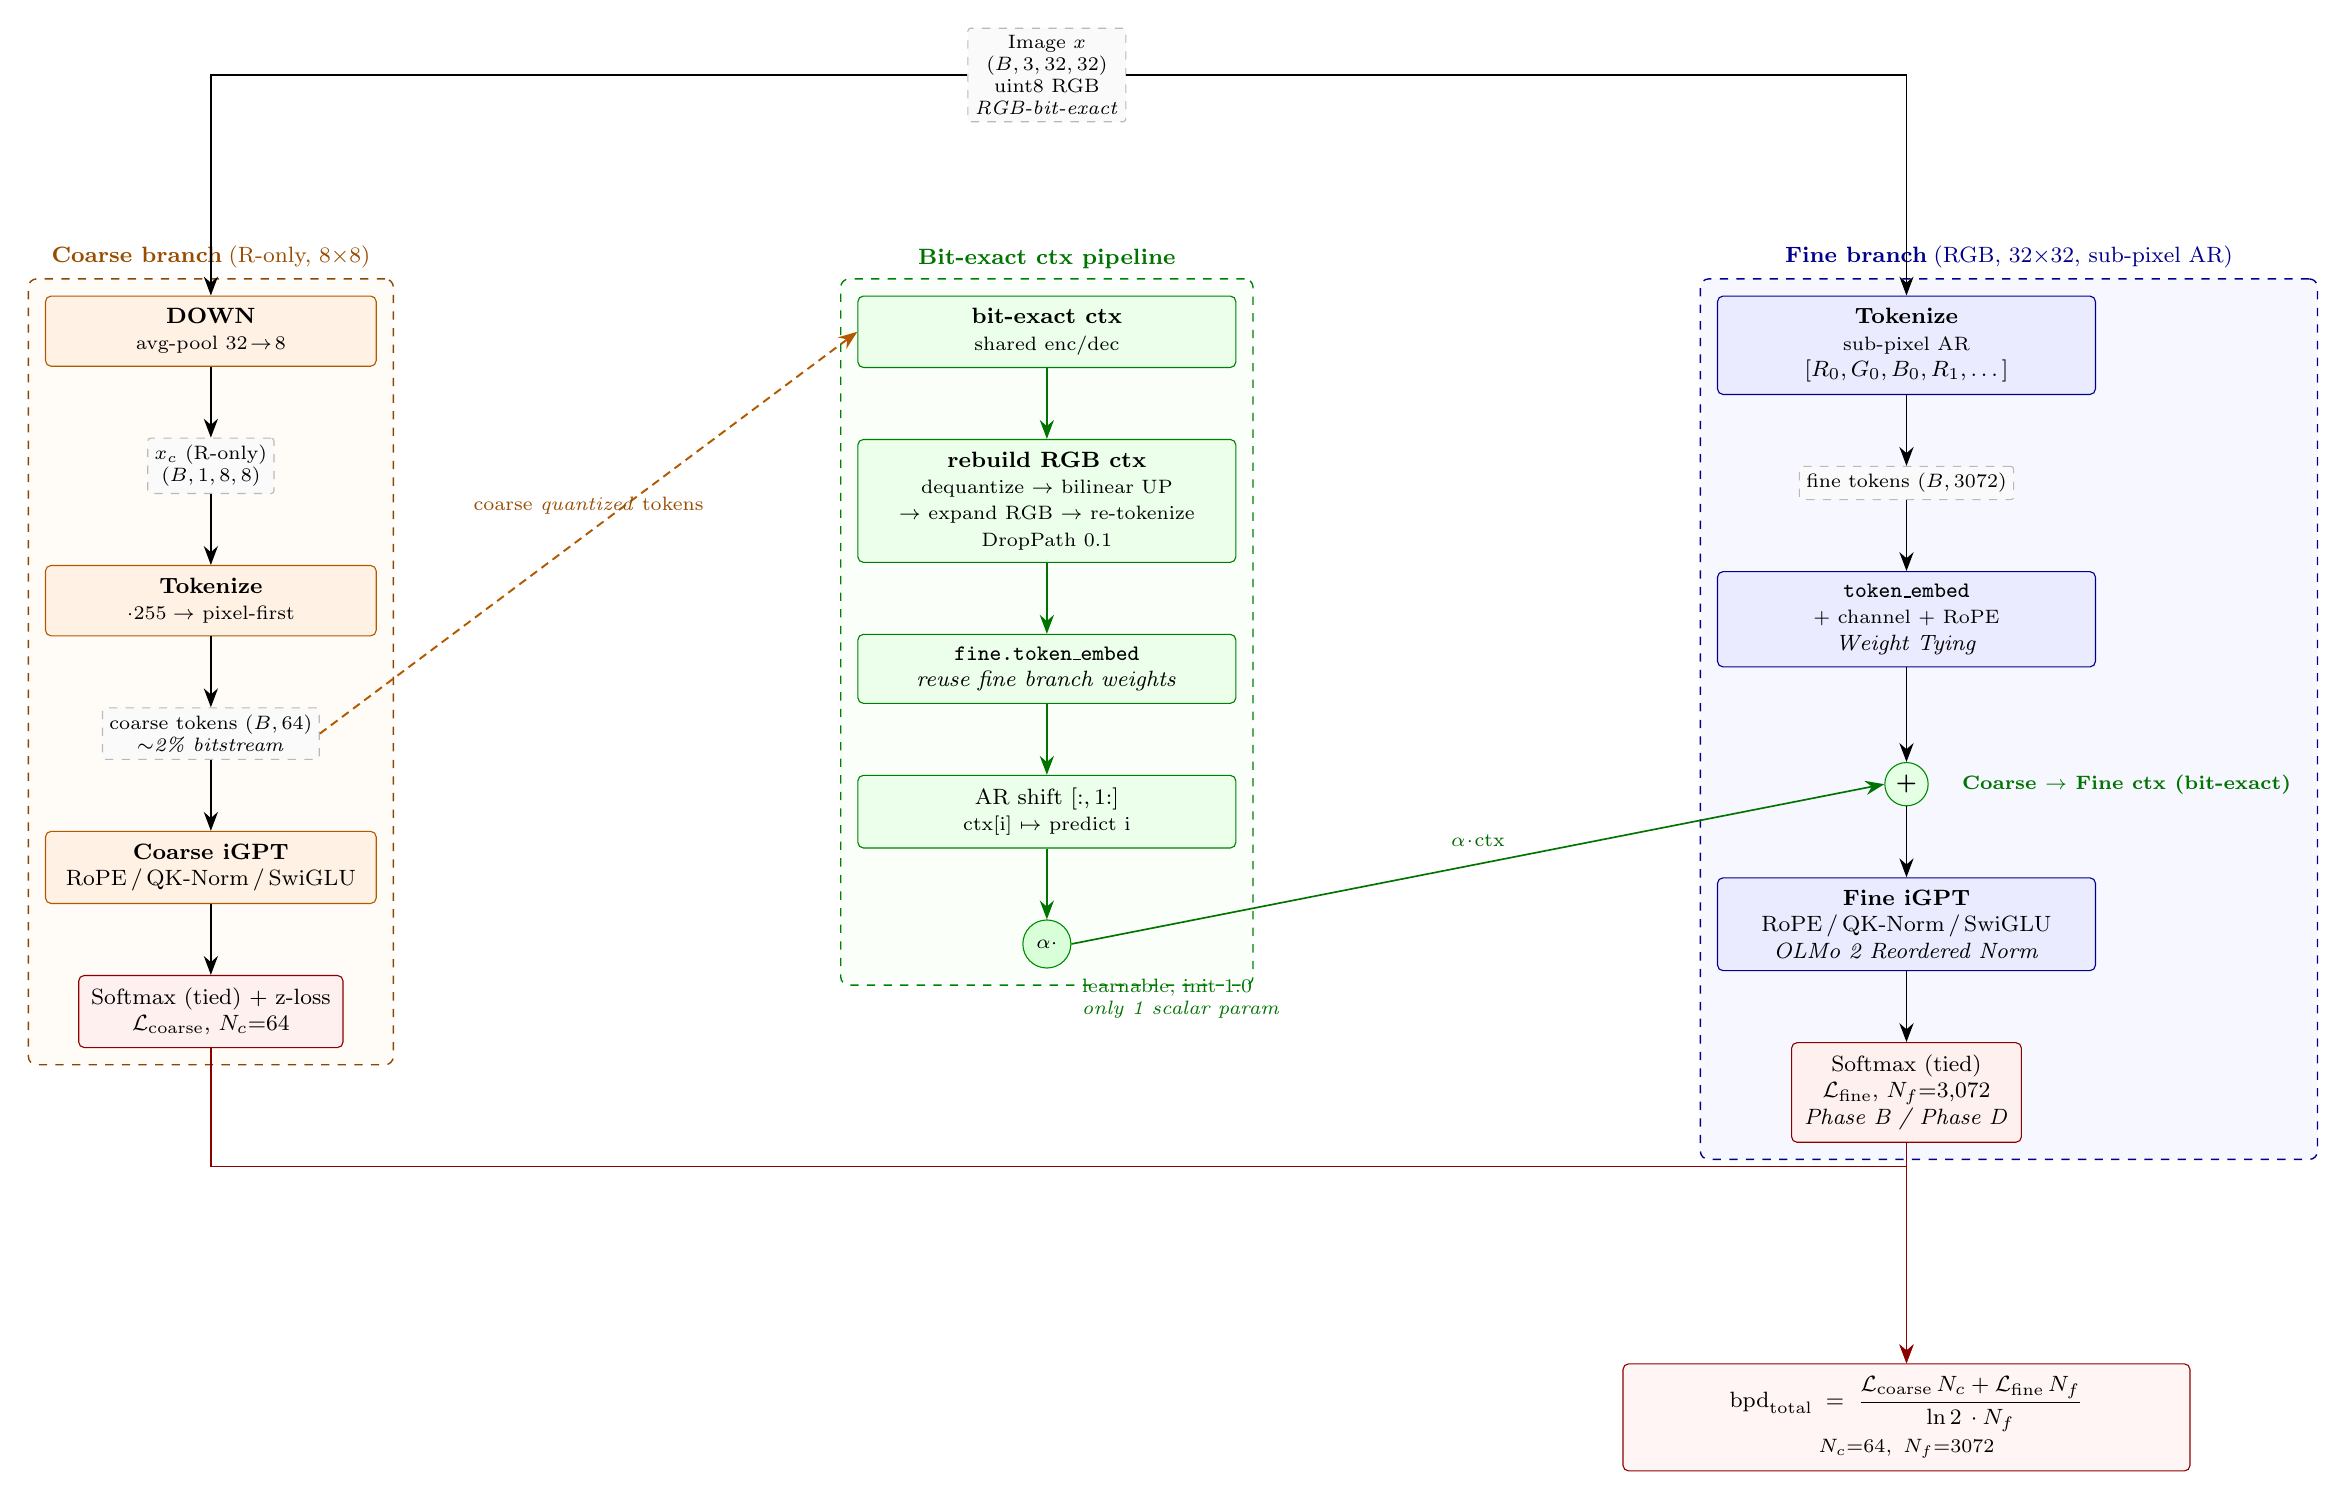
\begin{tikzpicture}[
    font=\footnotesize,
    >={Stealth[length=2.4mm]},
    node distance=9mm and 18mm, % 进一步优化间距
    % 模块样式
    blk/.style    ={draw, rounded corners=2pt, align=center,
                    minimum height=8mm, inner sep=4.5pt,
                    fill=blue!6, draw=blue!55!black, line width=0.4pt},
    coarseblk/.style={blk, fill=orange!10, draw=orange!70!black, minimum width=42mm},
    fineblk/.style  ={blk, fill=blue!8,   draw=blue!55!black,   minimum width=48mm},
    ctxblk/.style   ={blk, fill=green!8,  draw=green!50!black, minimum width=48mm},
    lossblk/.style  ={draw, rounded corners=2pt, align=center, fill=red!6,
                      draw=red!55!black, minimum height=8mm, inner sep=4.5pt},
    tensor/.style ={draw, dashed, rounded corners=1pt, align=center,
                    fill=gray!4, draw=gray!55, font=\scriptsize, inner sep=2.5pt},
    pillar/.style ={draw, rounded corners=3pt, dashed, line width=0.5pt,
                    inner sep=6pt}, % 增加pillar内边距
    flow/.style   ={->, line width=0.5pt},
    ctxflow/.style={->, line width=0.6pt, green!45!black},
    biteq/.style  ={->, line width=0.7pt, orange!70!black, densely dashed},
]

% ============================================================
% INPUT (顶部居中)
% ============================================================
\node[tensor] (x) {Image $x$\\$(B,3,32,32)$\\ uint8 RGB\\\textit{RGB-bit-exact}};

% ============================================================
% LEFT COLUMN — COARSE BRANCH (R-only 8x8)
% ============================================================
\node[coarseblk, below left=22mm and 75mm of x] (down)
    {\textbf{DOWN}\\\scriptsize avg-pool $32\!\to\!8$};

\node[tensor, below=of down] (xc)
    {$x_c$ (R-only)\\$(B,1,8,8)$};

\node[coarseblk, below=of xc] (ctok)
    {\textbf{Tokenize}\\\scriptsize$\cdot255 \to $ pixel-first};

\node[tensor, below=of ctok] (ctokens)
    {coarse tokens $(B,64)$\\\textit{$\sim$2\% bitstream}};

\node[coarseblk, below=of ctokens] (coarse)
    {\textbf{Coarse iGPT}\\
     RoPE\,/\,QK-Norm\,/\,SwiGLU};

\node[lossblk, below=of coarse] (cehead_c)
    {Softmax (tied) $+$ z-loss\\
     $\mathcal{L}_{\text{coarse}}$, $N_c{=}64$};

% ============================================================
% MIDDLE COLUMN — CTX PIPELINE (bit-exact) 【正中间】
% ============================================================
\node[ctxblk, below=22mm of x, xshift=0mm, align=center] (ctxstart)
    {\textbf{bit-exact ctx}\\\scriptsize shared enc/dec};
\node[ctxblk, below=of ctxstart] (rebuild)
    {\textbf{rebuild RGB ctx}\\
     \scriptsize dequantize $\to$ bilinear UP\\
     \scriptsize $\to$ expand RGB $\to$ re-tokenize\\
     \scriptsize DropPath 0.1};
\node[ctxblk, below=of rebuild] (embed)
    {\texttt{fine.token\_embed}\\\textit{reuse fine branch weights}};
\node[ctxblk, below=of embed] (shift)
    {AR shift $[:,1{:}]$\\\scriptsize ctx[i] $\mapsto$ predict i};

\node[draw, circle, fill=green!15, draw=green!55!black, minimum size=6mm,
      below=of shift] (alpha) {\scriptsize$\alpha\cdot$};
% 调整文字位置到alpha右下方
\node[font=\scriptsize, below right=1mm and 1mm of alpha, text=green!45!black, align=left]
     {learnable, init 1.0\\\textit{only 1 scalar param}};

% ============================================================
% RIGHT COLUMN — FINE BRANCH (32x32 sub-pixel AR)
% ============================================================
\node[fineblk, below right=22mm and 75mm of x] (ftok)
    {\textbf{Tokenize}\\\scriptsize sub-pixel AR\\$[R_0,G_0,B_0,R_1,\dots]$};

\node[tensor, below=of ftok] (ftokens)
    {fine tokens $(B,3072)$};

\node[fineblk, below=of ftokens] (tokemb)
    {\texttt{token\_embed}\\\scriptsize $+$ channel $+$ RoPE\\\textit{Weight Tying}};

% --- α 注入交汇点 ---
\node[draw, circle, inner sep=0.6pt, fill=green!10, draw=green!55!black,
      minimum size=5.5mm, below=12mm of tokemb] (plus) {$\boldsymbol{+}$};

% 关键修改：将标签放在绿色加号圆形的右边
\node[font=\scriptsize, right=3mm of plus, text=green!45!black, anchor=west]
     (ctxlabel) {\textbf{Coarse $\to$ Fine ctx (bit-exact)}};

\node[fineblk, below=of plus] (fine)
    {\textbf{Fine iGPT}\\
     RoPE\,/\,QK-Norm\,/\,SwiGLU\\\textit{OLMo 2 Reordered Norm}};

\node[lossblk, below=of fine] (cehead_f)
    {Softmax (tied)\\
     $\mathcal{L}_{\text{fine}}$, $N_f{=}3{,}072$\\\textit{Phase B / Phase D}};

% ============================================================
% BPD AGGREGATION (底部居中)
% ============================================================
\node[lossblk, fill=red!4, below=28mm of cehead_f, minimum width=72mm] (bpd)
    {$\displaystyle
        \mathrm{bpd}_{\text{total}}
        \;=\;\frac{\mathcal{L}_{\text{coarse}}\,N_c + \mathcal{L}_{\text{fine}}\,N_f}{\ln 2\,\cdot N_f}$
    \\[2pt]\scriptsize $N_c{=}64,\ N_f{=}3072$};

% ============================================================
% EDGES — main flow (彻底优化路径，无任何重叠)
% ============================================================
% input split
\draw[flow] (x) -| (down);
\draw[flow] (x) -| (ftok);

% coarse column
\draw[flow] (down)    -- (xc);
\draw[flow] (xc)      -- (ctok);
\draw[flow] (ctok)    -- (ctokens);
\draw[flow] (ctokens) -- (coarse);
\draw[flow] (coarse)  -- (cehead_c);

% fine column
\draw[flow] (ftok)    -- (ftokens);
\draw[flow] (ftokens) -- (tokemb);
\draw[flow] (tokemb)  -- (plus);
\draw[flow] (plus)    -- (fine);
\draw[flow] (fine)    -- (cehead_f);

% ctx bit-exact pipeline (关键修复：直接水平连接，无直角弯)
\draw[biteq] (ctokens.east) -- node[above,font=\scriptsize,orange!60!black, yshift=1mm]
            {coarse \emph{quantized} tokens}(ctxstart.west);
\draw[ctxflow] (ctxstart) -- (rebuild);
\draw[ctxflow] (rebuild)  -- (embed);
\draw[ctxflow] (embed)    -- (shift);
\draw[ctxflow] (shift)    -- (alpha);
% 只保留α·ctx标签在箭头上方
\draw[ctxflow] (alpha.east) -- node[above,font=\scriptsize,green!40!black, yshift=1mm]
              {$\alpha\!\cdot\!\mathrm{ctx}$} (plus.west);

% loss aggregation (关键修复：箭头直接指向block，无多余拐弯)
\draw[flow, red!55!black] (cehead_c.south) -- ++(0,-15mm) -| (bpd.north);
\draw[flow, red!55!black] (cehead_f.south) -- ++(0,-15mm) -| (bpd.north);

% ============================================================
% PILLAR BOXES (visual grouping)
% ============================================================
\begin{pgfonlayer}{background}
  \node[pillar, draw=orange!55!black, fill=orange!3,
        fit=(down)(xc)(ctok)(ctokens)(coarse)(cehead_c),
        label={[orange!60!black]above:\textbf{Coarse branch}\;(R-only, 8$\times$8)}]
        (coarsebox) {};
  \node[pillar, draw=green!50!black, fill=green!2, dashed,
        fit=(ctxstart)(rebuild)(embed)(shift)(alpha),
        label={[green!45!black]above:\textbf{Bit-exact ctx pipeline}}]
        (ctxbox) {};
  \node[pillar, draw=blue!55!black, fill=blue!3,
        fit=(ftok)(ftokens)(tokemb)(plus)(ctxlabel)(fine)(cehead_f),
        label={[blue!55!black]above:\textbf{Fine branch}\;(RGB, 32$\times$32, sub-pixel AR)}]
        (finebox) {};
\end{pgfonlayer}

\end{tikzpicture}
\end{document}